
This worksheet primarily deals with logical circuits and their relationship with logical expressions. Below is a helpful chart of commonly used logical gates and their associated logical expressions. Also, in terms of logical notation, $\oplus$ and $\iff$ will represent XOR and XNOR, respectively. NAND and NOR will be represented using $\uparrow$ and $\downarrow$, respectively.
 \begin{enumerate}
   \item \begin{figure}[ht]
    \centering
    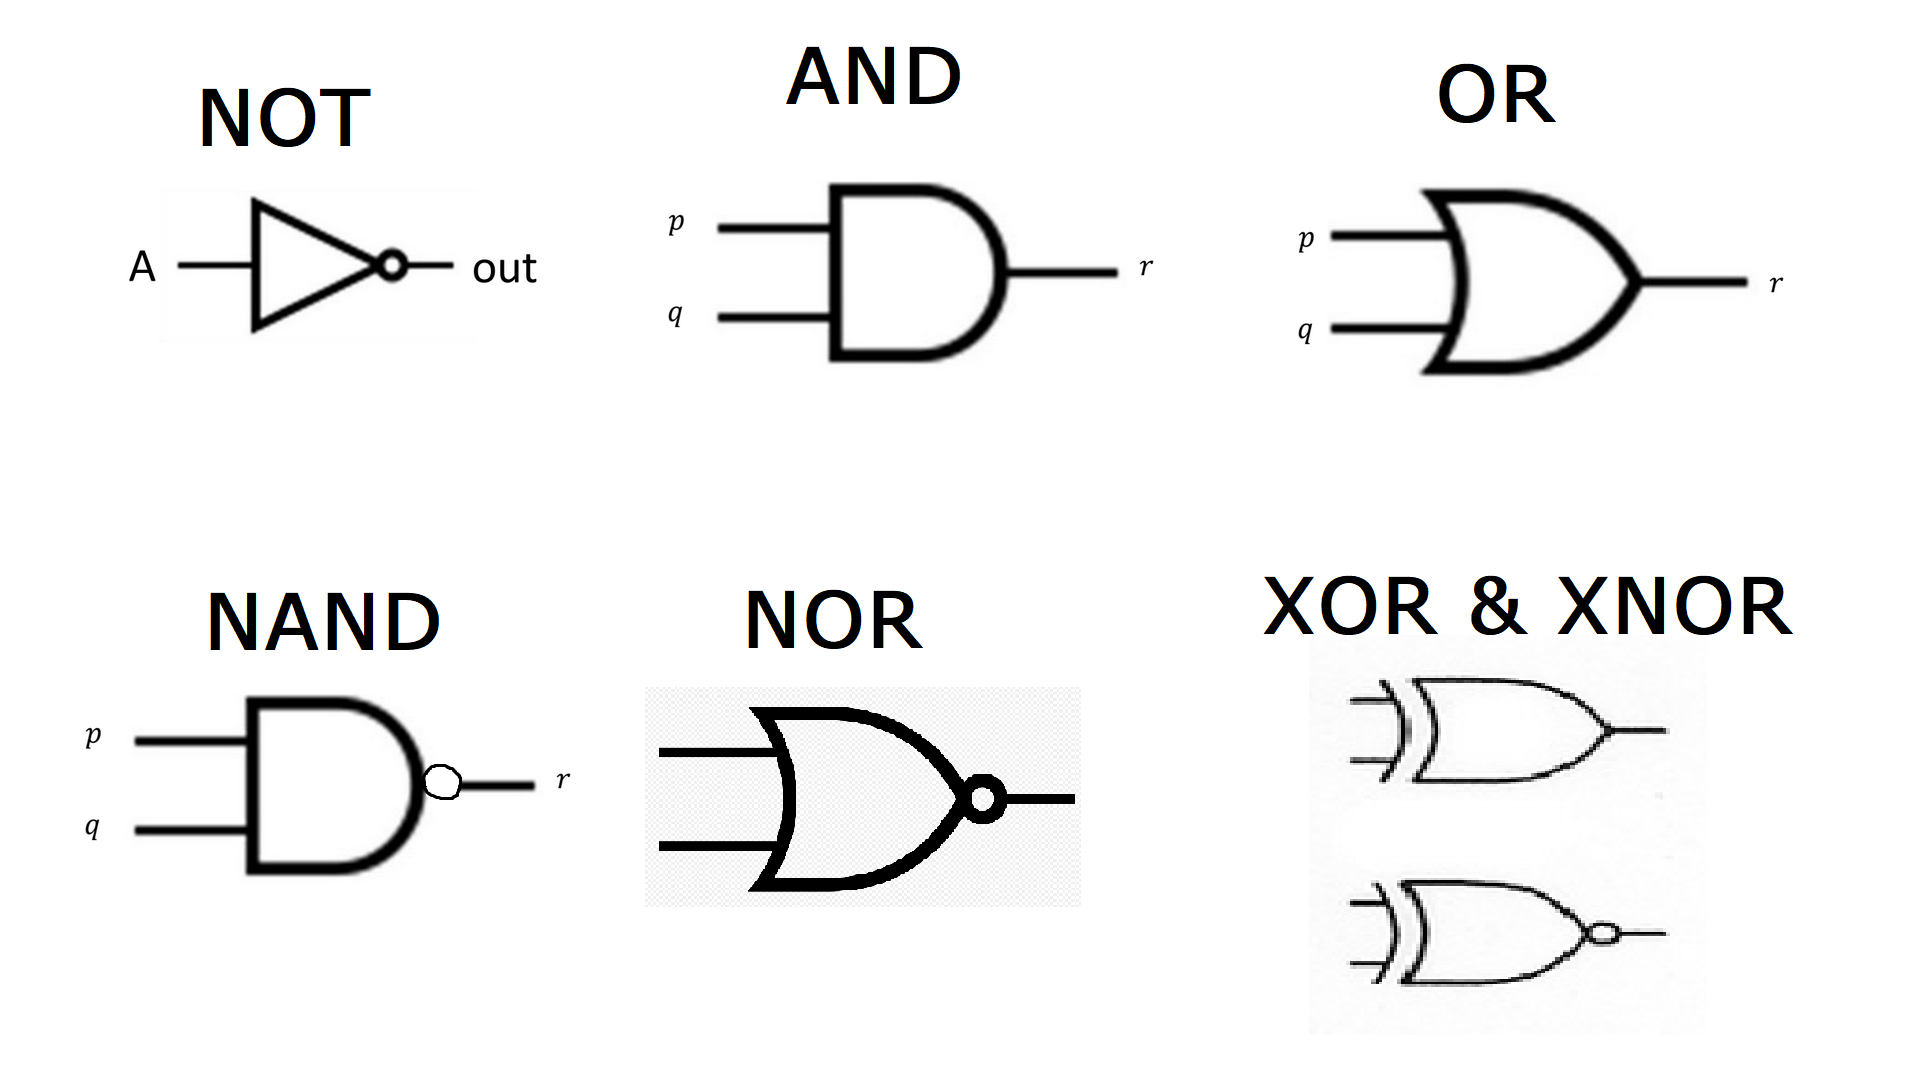
\includegraphics[width=\textwidth]{Ch2/circuit_ops.png}
    \caption{Circuit diagram gates}
    \label{fig:circ}
\end{figure}

The following question is a review from Thursday's lecture.

\begin{enumerate}
    \item Write $x \oplus y$ (XOR) using only the and ($\land$), or ($\lor$), and not ($\shortsim$) operations.
    \item Construct a circuit representing the boolean formula you wrote in part a).
\end{enumerate}
   \item For this problem and the next one assume that logic gates can take more than 2 inputs for inputs where they are \textbf{associative}. The reason why we require this is that some operators, such as NAND and NOR, are NOT associative and thus expressions like 
\[p \uparrow q \uparrow r\] are ambiguous.

Simplifying boolean expressions isn't all that useless! It seems to have ``applications'' in digital logic via the simplification of circuits, as discussed on circuit lecture. This problem is mostly a bunch of practice problems about this topic.

\begin{enumerate}
    \item Consider the logical expression $(r \lor ((s \lor q) \land r) ) \land (\shortsim (\shortsim (s \land q) )$.
    \begin{enumerate}
        \item Draw the circuit associated with this diagram.
        \item Simplify the logical expression above and draw an updated circuit associated with this diagram.
    \end{enumerate}
    \item Do the same thing, but for the logical expression $(a \land (\shortsim b)) \lor (a \land b)$.
    \pagebreak
    \item 
    \begin{enumerate}
    \item Okay, instead of converting a boolean formula into a circuit, convert this boolean circuit I made in mspaint to a boolean formula.
    
    \begin{figure}[ht]
        \centering
        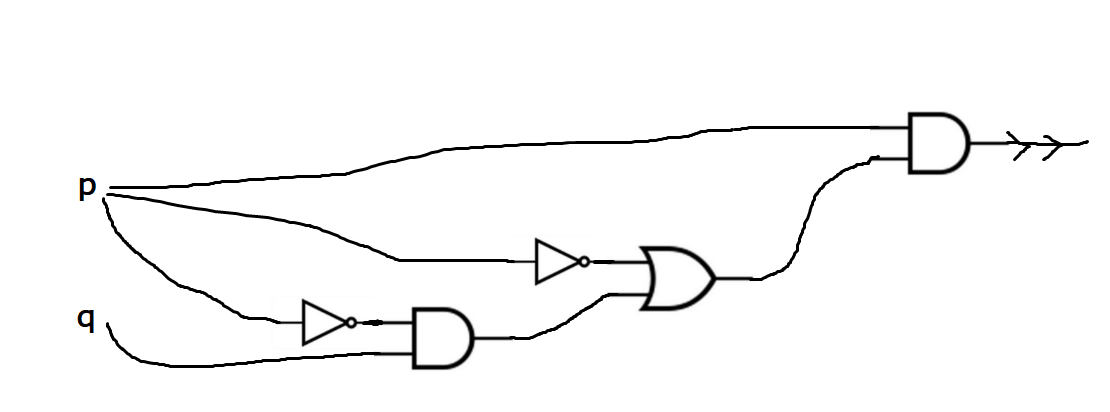
\includegraphics[width=\textwidth]{Ch2/002.png}
        \caption{Caption}
        \label{fig:my_label}
    \end{figure}
    
    \item Simplify this formula. After that, go ask around to see if there are any EE or CE majors in the room, because if you are not one of these people it is highly likely that you will not know how to draw the circuit for the simplified formula.
    \end{enumerate}
\end{enumerate}
   \item Assume for this problem that logic gates have a \textbf{cost} (just like in real life!). The cost list is below.

\begin{table}[H]
	\centering
	\renewcommand{\arraystretch}{1.2}
	\renewcommand{\tabcolsep}{2cm}
	\begin{tabular}{|c|c|} \hline 
		{\textbf{Gate}} & {\textbf{Cost}} \\ \hline
		NAND & 2 \\ \hline
		NOR & 4\\ \hline
		NOT & 3\\ \hline
		AND & 7\\ \hline
		OR & 3\\ \hline
		XOR & 6 \\ \hline
		XNOR & 11 \\ \hline
	\end{tabular}
	\caption{Some fictional gate costs.}
	\label{tbl:costs}
\end{table}
Suppose (for the sake of imagination) that this is the cost list for the fictional Alpha Beta Gamma computer hardware company. You are a consultant who is brought in to improve business pricing and advertising (although in this problem we will only focus on the pricing). Assume that people won't buy a gate if there is a cheaper alternative available. 

\begin{enumerate}
    \item The NAND gate is really, really cheap. (Actually, in real life, the NAND gate turns out to be the cheapest logic gate to construct, it requires the least transistors). Construct a NOT gate using the least number of NAND gates possible. Conclude if the current price for NOT is appropriate or not.
    
    \item Try to do the same thing for all the other logical gates and conclude whether or not their pricing is appropriate or not for each gate.
    
    \item (Challenge Problem, will probably not be discussed). Show that given any circuit, you can create an equivalent circuit using only the NAND gate. In other words, the NAND operator will generate any truth table. (Hint: what does the conjunctive normal form show?)
\end{enumerate}
 \end{enumerate}
